\documentclass{llncs}
%\usepackage{fancyhdr}
\pagestyle{plain}
%\pagestyle{headings}
\usepackage{standalone}
\usepackage{graphicx} 
\usepackage{comment}
%\usepackage{xcolor}
\usepackage{epigraph}
\usepackage{amsmath}
\usepackage{amsfonts}
\usepackage{amssymb}
\usepackage{cite}
%\usepackage{natbib}
%\usepackage[title]{appendix}
\usepackage{caption}
\usepackage{subcaption}
\usepackage{latexcolors}
\usepackage{import}
\usepackage{tikz}
\usetikzlibrary{positioning}
\usetikzlibrary {arrows.meta}

\newcommand{\red}[1]{\textcolor{red}{#1}}

\begin{document}

%


%\title{Telling the story of best friends}
%
\title{Best friends test: differential importance statistical test reveals hidden specific relations}
%
\titlerunning{Best friends test} 
% abbreviated title (for running head)
% also used for the TOC unless
% \toctitle is used
%
\author{
Alexandra Suvorikova \inst{1} \and Alexei Kroshnin \inst{1} \and Dmirijs Lvovs\inst{6} \and Vasily Ramensky \inst{2,3,4} \and Vera Mukhina \inst{5,6} \and Ludmila Danilova\inst{6} \and Andrey Mironov \inst{4,7} \and Alexander Favorov\inst{6,8}}
%
\authorrunning{A. Suvorikova et al.} % abbreviated author list (for running head)
%
%%%% list of authors for the TOC (use if author list has to be modified)
\tocauthor{Alexandra Suvorikova, Alexey Kroshnin, Dmitrijs Lvovs, Vasily Ramensky, Vera Mukhina, Ludmila Danilova, Andrey Mironov, and Alexander Favorov}
%
\institute{
Weierstrass Institute, Berlin, Germany, 
\email{suvorikova@wias-berlin.de}
\and
MSU Institute for Artificial Intelligence, \\Lomonosov Moscow State University, Moscow, 119992, RF
\and
National Medical Research Center for Therapy and Preventive Medicine of the Ministry of Healthcare of Russian Federation, Moscow, 101990, RF
\and
Department of Bioengineering and Bioinformatics, \\Lomonosov Moscow State University, Moscow, 119992, RF
\and
University of Maryland School of Medicine, Baltimore, MD 21205, USA
\and
Johns Hopkins University School of Medicine, \\ Baltimore, MD 21205, USA, \email{favorov@sensi.org}
\and
The Institute for Information Transmission Problems, Moscow, 127051, RF
\and
Vavilov Institute of General Genetics, RAS, Moscow, 119333, RF
}

\maketitle % typeset the title of the contribution

\renewcommand{\tag}{tag}
\newcommand{\collection}{collection}
\newcommand{\T}{T}
\newcommand{\C}{C}
\newcommand{\tl}{t}
\newcommand{\cl}{c}
\newcommand{\test}[1]{\textbf{\textit{#1}}}
%\setlength\epigraphwidth{.8\textwidth}
\setlength\epigraphrule{0pt}

\epigraph{SI AUGUSTUS CERNATUR, CERNANTUR QOUQUE AMICI}

\vspace{-0.2in}

\begin{abstract}
We propose a novel approach to select hidden specific relations in a dataset, which a bipartite graph can represent. 
To describe the hidden specific relations in general, we use a concept of \textit{friendship}. The goal is to detect objects in the data that are more important to particular others, than to the rest of the dataset, i.e. to detect friends. To this end, we introduce two statistical tests, the \test{best friend test} and the \test{friends test}. Both tests are based on the double ranking of the entries in the block of the weighted adjacency matrix of the bipartite graph. This model fits many practical problems, such as gene expression regulation by a set of transcription factors, etc. The method is available as an \textsf{R} package at \url{https://github.com/favorov/best.friends}.
\end{abstract}


\keywords{weighted bipartite graph, hidden relations, rank statistics, feature selection, clustering, knowledge transfer, specific gene regulation, pattern marker}

\section{Introduction: what it means to be a friend}

There is a simple intuition of what it means to be a friend. 
The friends of Augustus try to get together with him as often as possible. And if we meet August somewhere, we will likely meet his friends, too.

A similar setup arises if we analyze any observed data's inner relations. 
In the following, we model the relations as a bipartite graph. We numerically formulate the concept of friendship between graph nodes using a double-ranking procedure followed by a statistical test validating the ranking result. The approach detects specific relations in the data.

% A motivating example comes from the matrix factorization of omics data \cite{fertig_cogaps_2010, stein-obrien_enter_2018}. The factorization gives a matrix that shows the importance (the weights) of the features (e.g. expressions of particular genes) in biological processes.

A motivating example comes from omics data decomposition \cite{fertig_cogaps_2010, stein-obrien_enter_2018}. In this context, a matrix represents the decomposition. Its elements correspond to the weights that quantify the importance of specific \textcolor{red}{features} in \textcolor{red}{the observed biological processes} (e.g., the expression levels of particular genes). A feature is referred to as a \textit{marker} if it has substantial weight in only one process \cite{stein-obrien_patternmarkers_2017}.

The presence of a marker indicates the activity of the corresponding process. Conversely, features identified as noise or those with large weights across multiple processes should not be classified as markers. For instance, the work \cite{stein-obrien_patternmarkers_2017} aims to find all the markers and the corresponding marked processes. 

\paragraph{Approach} In our work, the detection of markers and marked processes is based on the concept of friendship: if a feature is a process marker, then the process is its friend.

This relationship is naturally modeled using a bipartite graph. The nodes in one set represent all observed features, while the nodes in the other set represent all biological processes. Weighted edges between these nodes indicate the degree of friendship.

% \textcolor{red}{For a given process, we identify its friend (marker) among the set of all other features.}

This setting applies to numerous problems. For the sake of generality, we refer to features as \textit{{\tag}s}, to processes as \textit{{\collection}s}, and to weights as \textit{attention}. See a corresponding bipartite graph at Fig.\ref{fig:nice_name}. The model applies to many setups (see Tab.\ref{tab:examples} for examples). 
\begin{figure}
 \centering
 \import{}{bipartite}
 \caption{Bipartite graph of tag-collection model. The attention $A(t, c)$ is the weight of an edge between node $c$ (collection) and node $t$ (tag).
 The arrows correspond to nonzero $A(t,c)$ .}
 \label{fig:nice_name}
\end{figure}

\begin{table}[h!]
\centering
\caption{Tag-collection model deployment examples.}
\label{tab:examples}
\begin{tabular}{c|c|c|c}
\textbf{Example} & \textbf{Tag $t$} & \textbf{Collection $c$} & \textbf{Attention $A(t, c)$} \\ 
\hline

\begin{tabular}[c]{@{}c@{}}Search engine\end{tabular} & Query & \begin{tabular}[c]{@{}c@{}} Search result \end{tabular} & \begin{tabular}[c]{@{}c@{}}Relevance of\\ search output\\\end{tabular} \\ \hline

\begin{tabular}[c]{@{}c@{}}Gene expression regulation\\ by transcription factors\end{tabular} & Gene & \begin{tabular}[c]{@{}c@{}}Genes under regulation \\ by the transcription factor \end{tabular} & \begin{tabular}[c]{@{}c@{}}Strength of \\ regulation\end{tabular} \\ \hline

\begin{tabular}[c]{@{}c@{}}Transcription\\ decomposition\end{tabular} & Transcript & \begin{tabular}[c]{@{}c@{}}Complex biological process\end{tabular} & \begin{tabular}[c]{@{}c@{}}Transcript's weights \\ in process\end{tabular} \\ \hline

\begin{tabular}[c]{@{}c@{}}Transcription \\ correlation\end{tabular} & Transcript & \begin{tabular}[c]{@{}c@{}}Another transcript\end{tabular} & \begin{tabular}[c]{@{}c@{}}Correlation of transcription values\\ measured in different experiments\end{tabular} \\ \hline
Fuzzy clustering & Object & Cluster & \begin{tabular}[c]{@{}c@{}}Object weight \\ in cluster\end{tabular} \\ \hline


\begin{tabular}[c]{@{}c@{}}Weighted graph\end{tabular} & Vertex & \begin{tabular}[c]{@{}c@{}} Another vertex \end{tabular} & \begin{tabular}[c]{@{}c@{}}Weight of edge between\\ collection and tag \end{tabular} \\ \hline
\end{tabular}
\end{table}

\paragraph{Our goal} For each tag $t$, we aim to find all ``friendly'' collections in $c$. Returning to the markers and processes example, we search among all tags for markers and the processes they label.


\subsection*{Blueprint of the procedure}
 

% \textcolor{red}{First, for a fixed tag, we range all collections by their ``friendliness''.} Then we carry out a statistical test to filter out noise, on the one hand, and nonspecific strong relations, on the other.

The proposed procedure \textcolor{red}{relies on some modeling assumptions} and consists of two steps. 
First, for each tag, we quantify the degree of friendliness associated with each collection. In the second step, we perform a statistical test to filter out both noise and nonspecific strong relationships.

\textbf{First step.} The quantification of friendliness is based on ranking. A straightforward approach might be to assume that the higher the attention a collection $c$ gives to a tag $t$, the more friendly the collection $c$ is to the tag $t$. However, this na\"ive method fails to differentiate between tags that are specific markers and those that receive high attention from all collections (e.g., so-called network hubs). So, we suggest a double-ranking approach. It points to the most friendly collection(s) for a given tag $t$. 

\textbf{Second step.} To select the true friends among all friendly collections, we use a statistical procedure based on some modeling assumptions. We name it the \test{friends test}. 

For a given tag $t$, the \test{friends test} splits the set of all collections into two subsets: the friends of the tag and all the others. 

It runs for only one tag of interest. Since we usually have no apriori preferences for a tag, we can run it for all the tags simultaneously. In this case, we should consider the multiplicity correction. 

\textbf{Computational aspects.} \textcolor{red}{the procedure is fast and suitable for large data sets!}

\textbf{R-package}
The software that implements the \text{best friend test} and \text{friends test} is available as an \textsf{R} package \textsf{best.friends} at 
\url{https://github.com/favorov/best.friends}. The vignette of the package shows simple usecases.


\paragraph{The organization of the paper} Section~\ref{sec:method} introduces the procedure in detail. \textcolor{red}{Section...}

\section{\textit{Friends}-method}
\label{sec:method}
Denote a set of all observed collections as $C := \{c_1, \dots, c_k\}$, and a set of all observed tags as $T := \{t_1, \dots, t_n\}$.
The attention $A(t_i, c_j)$ is the weight of an edge between $t_i$ in $ T$ and $c_j$ in $C$ (see Fig.\ref{fig:nice_name}).
Let's agree that the greater the $A(t_i, c_j)$, the higher the attention is. Naturally, the absence of attention corresponds to $A(t_i, c_j) = 0$. 

Let $a_{ij} := A(t_i, c_j)$. The corresponding attention matrix is 
\[
\mathcal{A} := \begin{pmatrix}
a_{11} & a_{12} & \dots & a_{1k} \\
 &\cdots & \cdots & \\
a_{n1} & a_{n2} & \dots & a_{nk}
\end{pmatrix}.
\]
Of note, one may think of $\mathcal{A}$ as a non-diagonal block of a weighted adjacency matrix of the bipartite graph.

In what follows we will denote the $i$-th row of the matrix $\mathcal{A}$ as $\text{row}_i(\mathcal{A})$ and its $j$-th column $\text{col}_j(\mathcal{A})$, i.e.,
\[
\text{row}_i(\mathcal{A}) := (a_{i1}, \dots, a_{ik}),
\quad
\text{col}_j(\mathcal{A}) := (a_{1j}, \dots, a_{nj}).
\]
In other words, a row $\text{row}_i(\mathcal{A})$ corresponds to attention that a tag $t_i$ receives from all collections in $C$; a column $\text{col}_j(\mathcal{A})$ corresponds to attention from a collection $c_j$ to all tags in $T$.

In the rest of the text, we assume that all $a_{ij}$ are independent random variables.

Further, under $H_0$ we assume that the attention that each collection $c_j$ from $C$ pays to all tags in $T$ is identically distributed. In other words, values in $\text{col}_j(\mathcal{A})$have the same distribution. We denote it as $P_j$. Typically, all distributions $P_1, \dots, P_k$ are unknown and may vary in nature. 

\subsection*{First step: double ranking}


For each collection $c_j \in C$, we decreasingly rank the elements inside $\text{col}_j(\mathcal{A})$. Thus, for each $a_{ij} $ in $\text{col}_j(\mathcal{A})$, we get the ordinal number $o_{ij}$. \textcolor{red}{We resolve the ties by the mean rank of the tied elements. (ties.method = random)} 

Let $\mathcal{O}$ denote the matrix containing ordinal numbers $o_{ij}$ in place of the corresponding attention values $a_{ij}$, 
\begin{equation*}
\mathcal{O} = \begin{pmatrix}
o_{11} & o_{12} & \dots & o_{1k} \\
 &\cdots & \cdots & \\
o_{n1} & o_{n2} & \dots & o_{nk}
\end{pmatrix}, 
\quad
o_{ij} :=\text{rank}\left(a_{ij}~ \text{inside}~\text{col}_j(\mathcal{A})\right).
\end{equation*}
As before, we denote the $i$-th row of $\mathcal{O}$ as $\text{row}_i(\mathcal{O}) := (o_{i1}, \dots, o_{ik})$.

To quantitatively express the friendliness of all collections to the fixed tag $t_i$, we decreasingly order the ranks stored in $\text{row}_i(\mathcal{O})$. Denote the corresponding rearrangement as $r_{i1}, \dots, r_{ik}$. By construction, $r_{i1} \le r_{i2} \le \dots \le r_{ik}$. Let the corresponding matrix be
\begin{equation}
\label{def:R}
\mathcal{R} := \begin{pmatrix}
r_{11} & r_{12} & \dots & r_{1k} \\
 &\cdots & \cdots & \\
r_{n1} & r_{n2} & \dots & r_{nk}
\end{pmatrix}.
\end{equation}
\paragraph{Idea behind the statistical test} To find the best friends of the tag $t_i$ we are going to split the items inside $\text{row}_{i}(\mathcal{R}) = (r_{i1}, \dots, r_{ik})$ into two non-intersecting groups. One group will match best friends and the other group will match all other collections. 

%NB! Сказать в дискуссии, что метод работает даже если модельное предположение ломается?
\subsection*{Second step: statistical test}
Keeping in mind that now we deal with a single tag $t_i$, let's, for simplicity, omit index $i$. Then, 
\[
\text{row}_{i}(\mathcal{R}) = (r_{1}, \dots, r_{k}), 
\quad
r_{1} \le \cdots \le r_{k}.
\]

Before proceeding, we must verify that the tag is not indifferent to all collections, e.g. to reject $H_0$. To do this, one can either use a test to assess the homogeneity of the sample $r_{1}, \cdots, r_{k}$ or, alternatively, apply an information criterion, which will be introduced later in the text (see paragraph \textit{Information Criterion})

Assuming a tag has at least one true friend, we aim to split all collections into two groups. A group containing best friends collections, i.e. the collections corresponding to $r_1, \dots, r_{s^*}$ and all the other.

Before introducing a statistical model, we recall two important facts. First, $r_{1}, \cdots, r_{k}$ are independent random variables. Second, each $r_l$ ($1\le l \le k$) takes value ranging from $1$ to $n$. This is because, by construction, each $r_l$ is an ordinal number.

Under $H_1$, we assume that each $r_l$ ($1\le l \le k$) comes from a mixture of two uniform distributions on the discrete grid $1, \dots, n$.
Specifically, the mixture consists of a uniform distribution supported on $1, \dots, m^*$, and a uniform distribution supported on $m^* + 1, \dots, n$, where $m^*$ is an unknown parameter. The probability of each $r \in \{1, \dots, m^*\}$ is $\frac{p^{*}}{m^*}$ and $r \in \{ m^*+1, \dots, n\}$ is $\frac{1 - p^{*}}{n - m^*}$,
see Fig.\ref{fig:model}.
\begin{figure}
 \centering
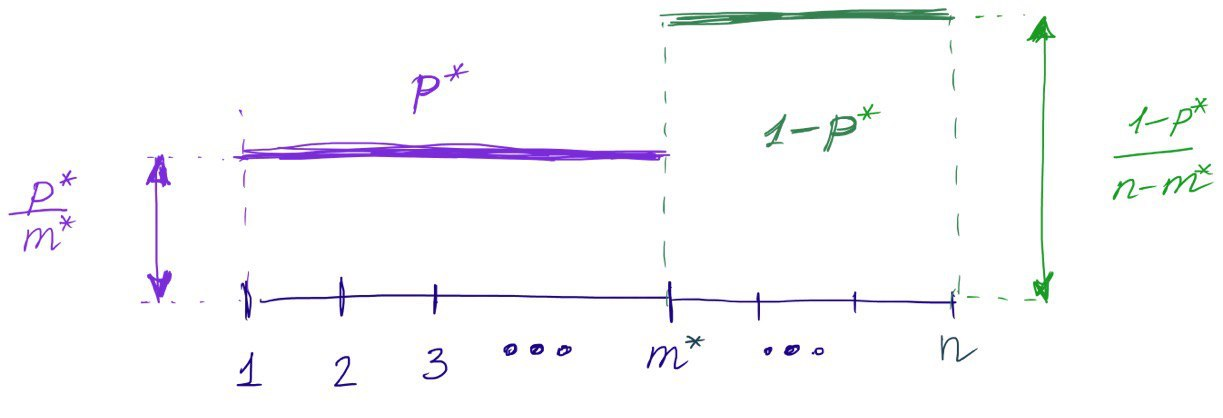
\includegraphics[width=0.8\textwidth]{model.jpeg}
 \caption{....}
 \label{fig:model}
\end{figure}

Note, that $p^*$ and $m^*$ are not known.
We use the maximum likelihood estimation to estimate them based on the observed data $r_1, \dots, r_k$. The likelihood of the mixture is
\[
L(p, m; r_1, \dots, r_k) := s\ln\left(\frac{p}{m}\right) + (k-s)\ln\left(\frac{1-p}{n - m}\right),
\quad
s: r_{s} \le m, ~r_{s+1} > m.
\]
The goal is to find $\hat{p}$ and $\hat{m}$ maximizing $L(p, m; r_1, \dots, r_k)$. Optimizing by $p$ ensures that $\hat{p} = \frac{s}{k}$. All aforementioned ensures that one can use brute-force search over $m$ to find the optimal parameters.

\paragraph{Information criterion}
One can avoid using the homogeneity test by applying the following information criterion.
The approach relies on some preliminary knowledge of the data. Specifically, one has to assume how likely it is that the tag $t$ has friends. We denote the corresponding probability as $q \in (0, 1)$ and set
\[
L_1 := L(\hat{p}, \hat{m}) + \ln(q),
\quad
L_2 := L(0, 0) + \ln(1-q).
\]
The best fit corresponds to $\max\{L_1, L_2\}$.



% \subsection{Symmetric attention matrix $\mathcal{A}$}
% % \textcolor{blue}{\textit{The matrix shows relation tags vs collection and it is not quadratic. How can the non-quadratic matrix be symmetric?}}
% It may happen that the number of tags $n$ coincides with the number of collections $k$, $n = k$. The particular case of the symmetric (by construction) attention matrix $\mathcal{A}$ requires a more detailed investigation.

% The $p$-value calculation relies on the assumption of the independence of attention values in different collections. If the attention matrix $\mathcal{A}$ is symmetric by the nature of the underlying bipartite graph, this assumption \textcolor{red}{does not hold}. Thus, the theoretical inference presented in Section~\ref{sec:theory} is not valid anymore.

% Still, the numerical procedure works. We show this in more detail in Supplement~\ref{seq:symmetric_a}. Of note, sometimes we know that all the diagonal elements are $0$ by construction. In this case, both tests use 
% \[
% p(w) = (1-w)^{k-1}, ~~\text{cf. equation \eqref{eq:pw}.}
% \]


\subsection{Multiple testing}
\label{sec:multimurkers}

All the tests we formulated here are not corrected for the multiplicity of hypotheses. Namely, they work directly if we \textit{a-priori} know what tag $t_i$ and what size $l$ of friends set we run the test for. 

In practice, the tests are run for each tag or even for each tag and the friend set population. Two important observations follow.

\paragraph*{Multiplicity correction} 
To run the \test{best friend test} on all the $n$ tags, we 
calculate $n$ $p$-values. To run the \test{friends test}, we calculate $n \cdot k$ $p$-values. However, all the tests rely on the ranking of the elements inside the same attention matrix $\mathcal{A}$. Thus, the assumption of test independence does not hold. In this case, the standard Bonferroni correction on the set of corresponding $p$-values is possibly too strong (\cite{cabin2000bonferroni}). However, some correction is still necessary. We leave it to the scope of the particular application.

\paragraph*{Multimarkers} Note that after the multiple hypothesis correction, a collection may be the best friend (or an element of the true friends set) for more than one tag. The set of tags is thus a multimarker for the collection. In practice, a multimarker tags (selects) a collection more specific than each of its elements.

\subsection{Friends and antagonists}





\section{Application examples}
\subsection{\red{Senteiment analysis}}
\paragraph{Data} To illustrate the performance of the 
\textbf{friends} test, we use AffectVec data \red{[cite]}. This is a word emotion database capturing the subtlety of the English language by providing over 70,000 words annotated with intensity scores for more than 200 emotions. AffectVec quantifies the degree to which each word evokes a wide range of emotional responses. For example, the word ``prank'' may primarily convey joy. Yet it can also be associated with fear, suspense, or a blend of other emotions.

AffectVec is organized as a tabular. Each row corresponds to an individual word and each column represents one of the more than 200 emotion categories. In other words, words are \textit{tags}, emotion categories are \textit{collections} and the corresponding intensity scores are \textit{attentions}. 

\paragraph{Data preprocessing} To test the \textbf{friends} test, we selected $1080$ adjectives (\red{using Python}). \red{Appendix} presents the selection procedure. The data is available at \red{url}.

\red{We consider two settings}: friends, anti-friends. Full list of emotions and manually filtered list of emotions.

Multiplicity correction: $\frac{1}{1080}$

\subsection{Experiment by AF...}
\section{Discussion}

In this manuscript, we develop a method and software to detect noteworthy edges in a weighted bipartite graph. We suppose all edges of the graph to be co-directed. The graph models a directed relation (referred to as attention) from the vertices of one part (collections) to the vertices of another part (tags).

Essentially, the method consists of two steps. First, we use a double-ranking approach to find the putative friends. Then, to validate the friendship hypothesis, we perform a novel statistical test that is distribution-free.

Along with the single collection procedure (\test{best friend test}), we suggest its extension for a subset of collections (\test{friends test}).

The \text{best friend test} is a particular case of the \test{friends test}, but we consider it separately in the software and, hence, in the methods. Namely, \test{friends test} has higher computational costs and it requires multiplicity correction even for one tag (Section \ref{sec:multimurkers}). In many cases, the \text{best friend test} is enough for practical applications. 

Although the problem looks abstract, its solution has numerous straightforward applications. For instance, the detection of the marker genes \cite{stein-obrien_patternmarkers_2017} for expression patterns critically simplifies the biological interpretation of the results of transcription matrix factorization \cite{Stein_2018,Fertig_2016}. Here, the genes are tags and the patterns are collections. If a pattern is a friend of a gene (see Section \ref{sec:method}), the gene is the marker of the pattern.

However, the theoretical result is limited to the case of an asymmetric attention matrix. If the matrix is symmetric by the design, the null hypothesis does not hold. However, the computational experiment \textcolor{red}{(see Supplement)} shows that the independence proposition \textcolor{red}{can be used}. Thus, the method applies to the analysis of, e.g., distance matrices. 

The first possible area of application is feature selection. By identification of markers, instead of all tags, we can use a relatively small subset for further analysis. Moreover, the identification of friend-marker pairs helps to remove non-specific connections from a graph. 

Second, the proposed method is useful for efficient clustering of a set of selected features. Also, the friendship concept provides a new similarity measure that possibly generates more interpretable clustering, than the clustering with $\mathcal{A}$ being a similarity measure.

Another possible direction is knowledge transfer: if we know something new about Augustus, we know something new about his friends. 
\subsection{}


% \textcolor{blue}{+ Friedman test }
% %\url{https://en.wikipedia.org/wiki/Friedman_test}


\section{Conflict of interest}
The authors declare no conflict of interest.

\section{Acknowledgements}
AF acknowledges support by National Institutes of Health (NIH) P30CA006973 and 1U01CA253403-01.
Thanks to Daniel Shu and Caedmon Haas for the translation of the motto to gold Latin. 

\bibliography{gene-best-friends}

\bibliographystyle{splncs03}
%\begin{subappendices}

\newcommand{\beginsupplement}{%
 \setcounter{table}{0}
 \renewcommand{\thetable}{S\arabic{table}}%
 \setcounter{figure}{0}
 \renewcommand{\thefigure}{S\arabic{figure}}
 \setcounter{equation}{0}
 \renewcommand{\theequation}{S\arabic{equation}}%
 }

\newpage
\section*{Supplement}
\beginsupplement
\subsection{Data preprocessing} 
The full list of emotion categories used in the experiment is following:
\textit{joy, surprise, trust, anticipation, fear, anger, sadness, disgust, happiness, levity, hate, loyalty, melancholy, anxiety, embarrassment,  regard, stress, gusto, compunction, cynicism, situation, umbrage, favor, meekness, compassion, withdrawal, scare, unrest, calm, courage, despair, fidget, shyness, apathy, hysteria, shadow, resentment, optimism, heartstrings, bonheur, dudgeon, merriment, hope, foreboding, envy, interest, relaxed, cruelty, helplessness,   solicitude, satisfaction,   suspense, fondness, dolor, weakness, electricity, esteem, woe, relieved, wonder, attachment, pessimism, malice, love, compatibility, timidity, blessedness, exultation, tumult, alienation, humility, powerlessness, complacency, gloom, aggression, sensation, antipathy, gloat, doubt, empathy, consciousness, ingratitude, hopelessness, signal, alarm, dislike, stir, distance, smugness, repentance, easiness, friendliness, gravity, displeasure, discouragement, pique, benevolence, chagrin, tension, togetherness, panic, eagerness, pleasure, excitement, mood, animosity, defeatism, worship, repugnance, grudge, euphoria, antagonism, trait, brotherhood, stewing, pity, daze, sympathy, annoyance, encouragement,  buoyancy, devotion, triumph, contempt, belonging, sinking, unhappiness, trepidation, admiration, disapproval, indifference, affection, astonishment, oppression, languor, coolness, liking, behaviour, peace, misogyny, bang, cheerfulness, creeps, agitation, boredom, gratification  hurt, agape, concern, ardor, mourning, harassment, contentment, closeness, surprised, confusion, presage, approval, state, wrath, dander, reverence, content, amusement, indignation, fearlessness, depreciation, expectation, tenderness, misery, depression, forgiveness, willies, fit, comfort, shame, apprehension   delight, jealousy, aggravation, chill, warpath, serene, exuberance, resignation, gratitude, despondency, nirvana, lividity, emotion, disappointment horror, grief, weight, distress, intoxication, irritation, insecurity, pride, fever, rejoicing, impatience, politeness, tranquillity, hilarity, fury, gladness, thing, nausea, calmness, fulfillment, ecstasy, elation, playfulness, exhilaration, titillation, gratefulness, diffidence, radiance, sorrow, confidence, security, ego, hostility, frustration, attrition, angst, shock, preference, enthusiasm, isolation, conscience, scruple, worry, earnestness, malevolence, awe, guilt, identification.}



The filtered list of emotions
\textit{joy, happiness, surprise, gratitude, friendliness, hope, admiration, love, cheerfulness, trust, interest,
compassion, stress, fear, anger, sadness, hate, melancholy, anxiety, despair, powerlessness, aggression, dislike, cynicism, unrest, apathy, hysteria, calm, courage, shyness, 
 optimism, helplessness, weakness, pessimism, humility, antipathy, 
 togetherness, panic, eagerness, pleasure, excitement, euphoria, brotherhood, sympathy, annoyance, triumph, belonging, unhappiness, admiration, disapproval, indifference, affection, astonishment, 
 agitation, boredom, gratification, concern, harassment, contentment, closeness, confusion, approval, amusement, indignation, fearlessness, depreciation, expectation, 
 tenderness, misery, depression, forgiveness, fit, comfort, shame, apprehension, delight, jealousy, aggravation, chill, disappointment, horror, grief, distress, intoxication,
 irritation, insecurity, pride, impatience, politeness, tranquillity, calmness, playfulness, gratefulness, sorrow, confidence, security, ego, frustration, shock, enthusiasm, isolation, worry, guilt.}






\end{document}


